% Performance Comparison Charts
% Compile: pdflatex performance-comparison.tex

\documentclass[tikz,border=10pt]{standalone}
\usepackage{pgfplots}
\pgfplotsset{compat=1.18}
\usepackage{tikz}

\begin{document}

% FPS Comparison
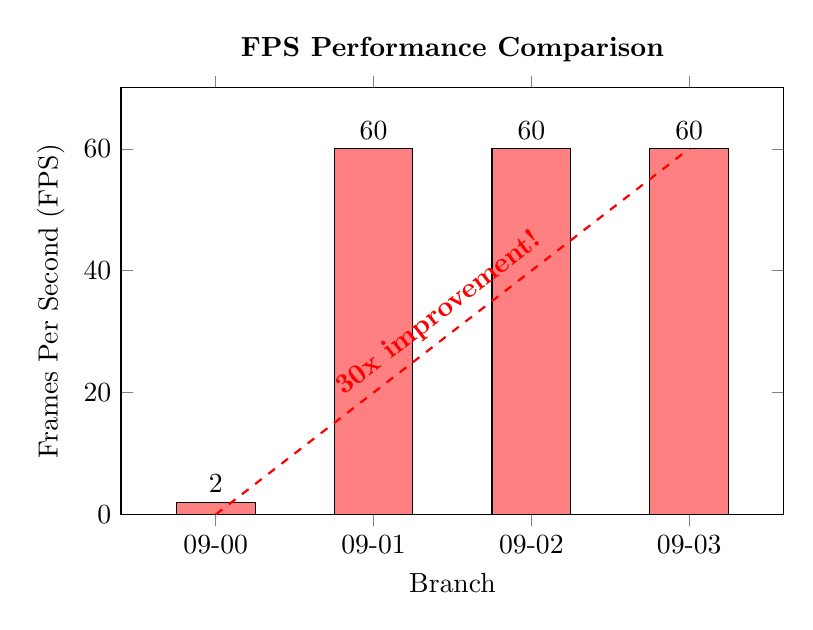
\begin{tikzpicture}
    \begin{axis}[
        ybar,
        width=10cm,
        height=7cm,
        ylabel={Frames Per Second (FPS)},
        xlabel={Branch},
        symbolic x coords={09-00,09-01,09-02,09-03},
        xtick=data,
        ymin=0,
        ymax=70,
        bar width=1cm,
        nodes near coords,
        nodes near coords align={vertical},
        title={\textbf{FPS Performance Comparison}},
        legend style={at={(0.5,-0.15)},anchor=north,legend columns=-1},
        enlarge x limits=0.2
    ]
        \addplot[fill=red!50] coordinates {
            (09-00,2)
            (09-01,60)
            (09-02,60)
            (09-03,60)
        };
        \draw[red,thick,dashed] (axis cs:09-00,0) -- (axis cs:09-03,60) node[midway,above,sloped] {\textbf{30x improvement!}};
    \end{axis}
\end{tikzpicture}

\vspace{1cm}

% Lines of Code in Main
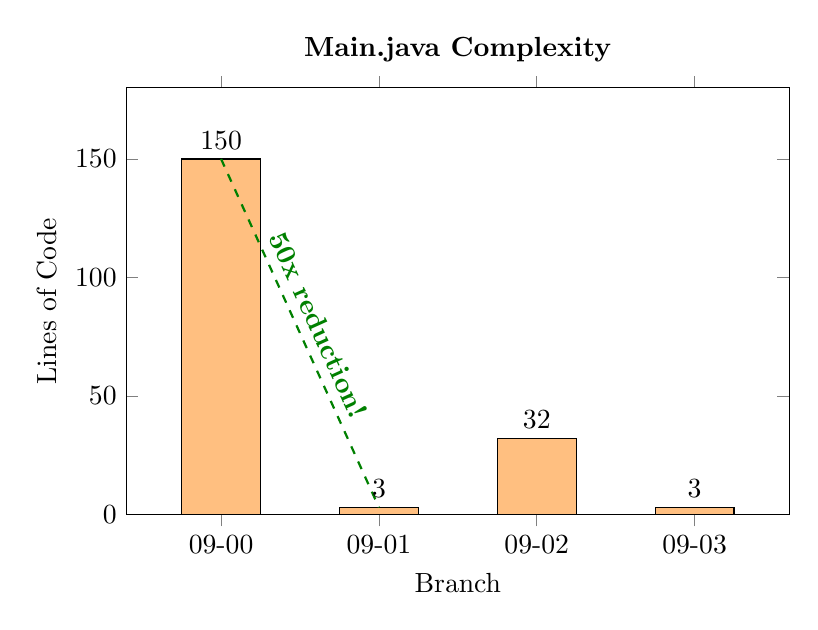
\begin{tikzpicture}
    \begin{axis}[
        ybar,
        width=10cm,
        height=7cm,
        ylabel={Lines of Code},
        xlabel={Branch},
        symbolic x coords={09-00,09-01,09-02,09-03},
        xtick=data,
        ymin=0,
        ymax=180,
        bar width=1cm,
        nodes near coords,
        nodes near coords align={vertical},
        title={\textbf{Main.java Complexity}},
        enlarge x limits=0.2
    ]
        \addplot[fill=orange!50] coordinates {
            (09-00,150)
            (09-01,3)
            (09-02,32)
            (09-03,3)
        };
        \draw[green!50!black,thick,dashed] (axis cs:09-00,150) -- (axis cs:09-01,3) node[midway,above,sloped] {\textbf{50x reduction!}};
    \end{axis}
\end{tikzpicture}

\vspace{1cm}

% Constructor Parameters Count
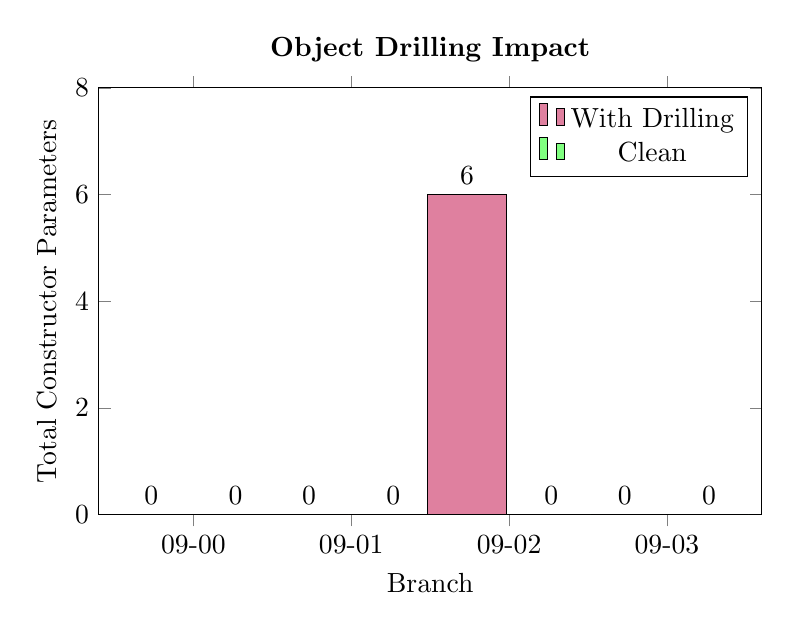
\begin{tikzpicture}
    \begin{axis}[
        ybar,
        width=10cm,
        height=7cm,
        ylabel={Total Constructor Parameters},
        xlabel={Branch},
        symbolic x coords={09-00,09-01,09-02,09-03},
        xtick=data,
        ymin=0,
        ymax=8,
        bar width=1cm,
        nodes near coords,
        nodes near coords align={vertical},
        title={\textbf{Object Drilling Impact}},
        enlarge x limits=0.2
    ]
        \addplot[fill=purple!50] coordinates {
            (09-00,0)
            (09-01,0)
            (09-02,6)
            (09-03,0)
        };
        \addplot[fill=green!50] coordinates {
            (09-00,0)
            (09-01,0)
            (09-02,0)
            (09-03,0)
        };
        \legend{With Drilling, Clean}
    \end{axis}
\end{tikzpicture}

\vspace{1cm}

% GameManager Instances Count
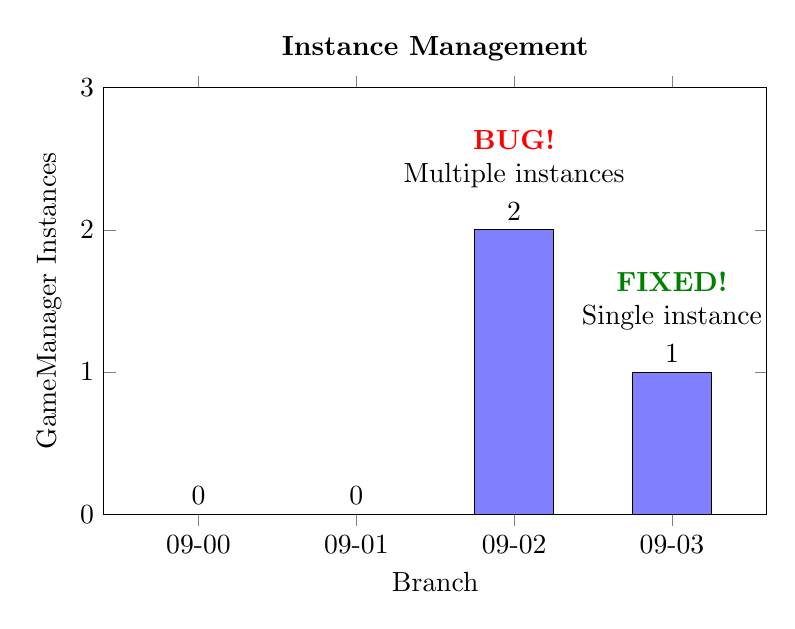
\begin{tikzpicture}
    \begin{axis}[
        ybar,
        width=10cm,
        height=7cm,
        ylabel={GameManager Instances},
        xlabel={Branch},
        symbolic x coords={09-00,09-01,09-02,09-03},
        xtick=data,
        ymin=0,
        ymax=3,
        bar width=1cm,
        nodes near coords,
        nodes near coords align={vertical},
        title={\textbf{Instance Management}},
        enlarge x limits=0.2,
        ytick={0,1,2,3}
    ]
        \addplot[fill=blue!50] coordinates {
            (09-00,0)
            (09-01,0)
            (09-02,2)
            (09-03,1)
        };
        \node[align=center] at (axis cs:09-02,2.5) {\textcolor{red}{\textbf{BUG!}} \\ Multiple instances};
        \node[align=center] at (axis cs:09-03,1.5) {\textcolor{green!50!black}{\textbf{FIXED!}} \\ Single instance};
    \end{axis}
\end{tikzpicture}

\vspace{1cm}

% Testability Score
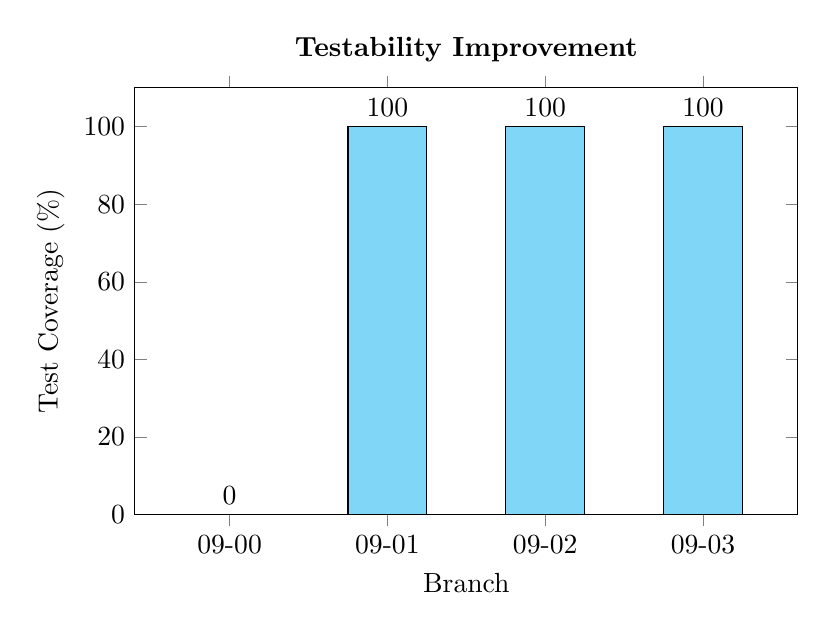
\begin{tikzpicture}
    \begin{axis}[
        ybar,
        width=10cm,
        height=7cm,
        ylabel={Test Coverage (\%)},
        xlabel={Branch},
        symbolic x coords={09-00,09-01,09-02,09-03},
        xtick=data,
        ymin=0,
        ymax=110,
        bar width=1cm,
        nodes near coords,
        nodes near coords align={vertical},
        title={\textbf{Testability Improvement}},
        enlarge x limits=0.2
    ]
        \addplot[fill=cyan!50] coordinates {
            (09-00,0)
            (09-01,100)
            (09-02,100)
            (09-03,100)
        };
    \end{axis}
\end{tikzpicture}

\end{document}
